%
% File acl2015.tex
%
% Contact: car@ir.hit.edu.cn, gdzhou@suda.edu.cn
%%
%% Based on the style files for ACL-2014, which were, in turn,
%% Based on the style files for ACL-2013, which were, in turn,
%% Based on the style files for ACL-2012, which were, in turn,
%% based on the style files for ACL-2011, which were, in turn, 
%% based on the style files for ACL-2010, which were, in turn, 
%% based on the style files for ACL-IJCNLP-2009, which were, in turn,
%% based on the style files for EACL-2009 and IJCNLP-2008...

%% Based on the style files for EACL 2006 by 
%%e.agirre@ehu.es or Sergi.Balari@uab.es
%% and that of ACL 08 by Joakim Nivre and Noah Smith

\documentclass[11pt]{article}
\usepackage{acl2015}
\usepackage{times}
\usepackage{url}
\usepackage{latexsym}
\usepackage{graphicx}


%\setlength\titlebox{5cm}

% You can expand the titlebox if you need extra space
% to show all the authors. Please do not make the titlebox
% smaller than 5cm (the original size); we will check this
% in the camera-ready version and ask you to change it back.


\title{Siamese Recurrent Architecture for Lyrical Similarities}

\author{Rohit Nair \\
  University of California, Berkeley \\
  {\tt rohit.nair@berkeley.edu} \\}

\date{}

\begin{document}
\maketitle
\begin{abstract}
  We present a siamese network architecture based on Long Short Term 
  Memory (LSTM) for analyzing pairwise lyrical similarity between 
  songs of varying length. The model shows promising results in understanding
  semantic relationships between songs. When compared to bag of words 
  based implementations, the neural network based model show significantly 
  better results. Even with a small dataset the model is able to learn
  similarities across genres which opens up opportunities to generate 
  recommendations that contrast with audio features as well as those
  that span languages.
\end{abstract}

\section{Introduction}

Recommendations has been an integral part of how humans navigate the world.
Whether it's word of mouth suggestions or real-time news feeds, 
recommendation engines are present all around us and cast their influence
in subtle and powerful ways. Song recommendations has been particularly
popular field for a long time as evident from the number of radio stations
in existence. Most of them are genre based, ie. they play songs from a 
particular genre and rarely cross over to another genre. This resulted in 
a lack of understanding of interplay among songs of different genre. That
was until the advent of music streaming services such as Pandora. Allowing
users to curate their own list of channels to listen to and letting them
express their likes and dislikes which opened the doors to a richer
understanding of songs.

There have been numerous studies performed using audio signals and lyrics to 
analyze song similarities with moderate success. Songs are an end product 
of a creative journey where layers of abstractions, metaphors, rhymes are 
added making the underlying theme hard to decipher at times even for a human 
subject. Hence calculating lyrical similarity using traditional n-gram 
models is inefficient due to the loss in semantic understanding. One way
this was avoided was by the use of collaborative filtering [citation]. 
Collaborative filtering looks at user's listening pattern to derive song's
feature by factorizing the matrix which maps user and songs. This approach
has been widely successful in Netflix competition and widely used in
providing product recommendations on e-commerce and content sites. Although
extremely effective, it suffers from a few drawbacks. Firstly, it requires
a large amount of user-product data to perform feature extraction which limits 
the problem domains where this could be applied. Secondly, it suffers from a 
self-fulfilling bias where it recommends a popular song as it's 
common in the mapping data which in turn makes the song even more common
resulting in even more recommendation.

With the advancements in neural networks and back propagation techniques,
there has been great strides made in using these models for generating 
semantic understanding and other natural language processing task. Of note
is the work by Mikolov et al. (2013) in representing word analogies in
vector space. Following the success of word embedding, many models were
created for representing documents and bodies of text in vector space. For
one the success of these models can be attributed to their ability to 
process text of variable length and eschew limitation of Markov models namely
the length of context it can remember. An RNN achieves this by passing
a hidden state $h_t$ forward at each time step $t \in {1,...,T}$ for data 
sequence $(x_1,...,x_T)$ as
\[ h_t = f(Wx_t + Uh_{t-1} ) \]
\begin{figure}
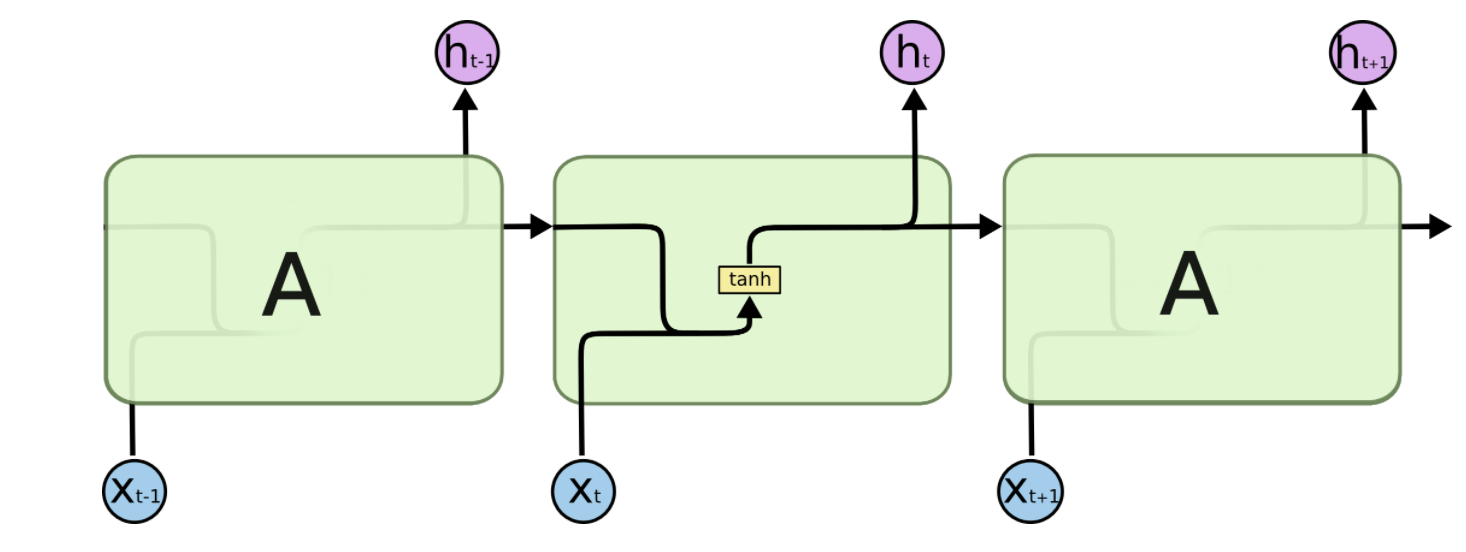
\includegraphics[width=\linewidth]{olahrnn.png}
\caption{A Recurrent Neural Network [ref Chris Olah]}
\end{figure}
where $f$ is a nonlinearity such as tanh or sigmoid.
A drawback of RNN is difficulty in optimizing the weights due to the
issue of vanishing gradients during backpropagation. LSTMs improve over
RNNs by managing to retain context over long sequence of inputs using
memory cells while maintaining a hidden state that is passed across the
units. An LSTM cell consists of 4 main components as shown in the figure 
below.
\begin{figure}
  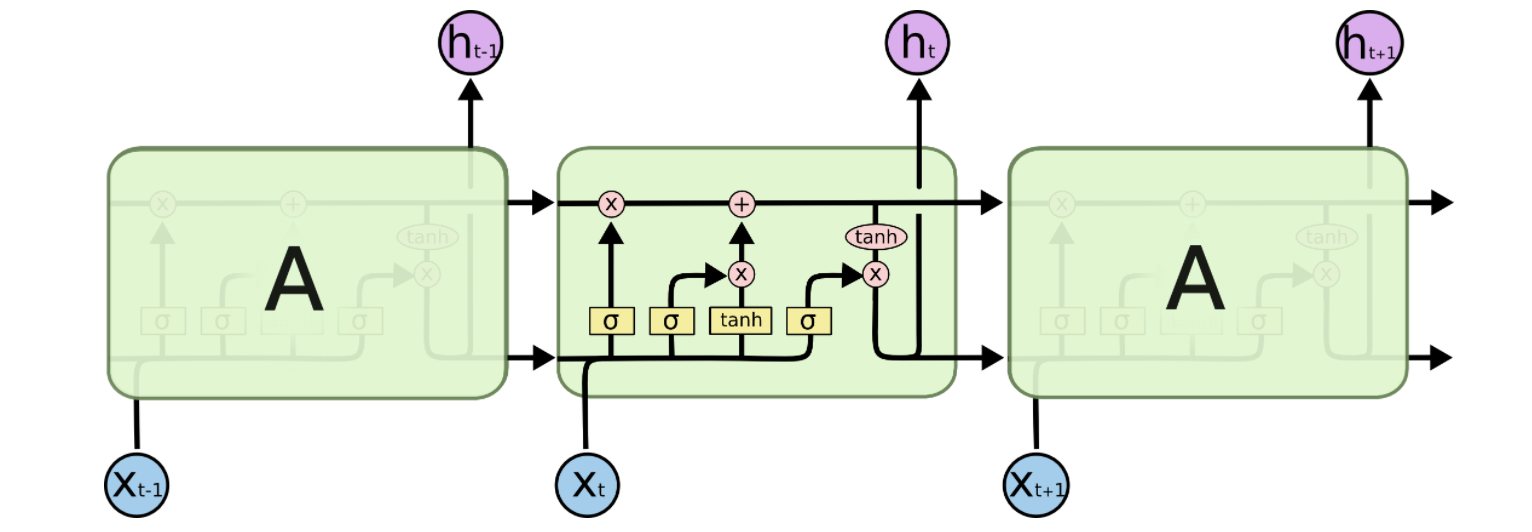
\includegraphics[width=\linewidth]{olahlstm.png}
  \caption{A Long Short Term Memory [ref Chris Olah]}
  \label{fig:lstm}
\end{figure}
The input gate, a sigmoid layer, decides which values we will update.
\[ f_t = \sigma(W_f[h_{t-1}, x_t] + b_f)\]

Next is a gate that decides which values to keep.
\[ i_t=\sigma(W_i[h_{t-1},x_t] + b_i)\]
\[ \tilde{C}_t = tanh(W_c[h_{t-1},x_t] + b_C)\]

We update the cell state based on above values as:
\[ C_t=f_t*C_{t-1} + i_t*\tilde{C}_t \]

Finally we decide what part of the cell data to send out as output.

\[ o_t= \sigma (W_o[h_{t-1}, x_t] + b_o) \]

\[ h_t=o_t*tanh(C_t) \]

The final output of the LSTM network encapsulates fragments of the 
inputs it encountered. Training is performed by means of backpropagation
where the error is propagated back through the cells to modify these
trainable weights.

In this work we adapt the Siamese recurrent neural network proposed by
Mueller et al (2016) to the task for lyrical similarity analysis. The
model accepts as input pairs of song lyrics $(x^{(a)}_{i},....x^{(a)}_{T_a}),
(x^(b)_{i},....x^(b)_{T_b})$ of fixed-size vectors (each $x^{(a)}_i,x^{(b)}_j
\in R^{d_in}$ along with a label $y$ that represents the similarity 
between the songs. The model generates a mapping from general space of 
variable length sequence to structure matrix space of fixed dimensionality.
Post training, a new song lyrics could be passed through this model so
as to generate it's matrix representation.



\section{Model}
The Manhattan LSTM (MaLSTM) as proposed by Mueller et al is shown in the 
figure below. Manhattan here stands for the Manhattan distance between 
the two song's matrix representations. In our case we use the 
Euclidian distance as a measure of similarity. We feed the lyrics of
the songs to the LSTM for it to update the hidden state at each sequence.
The final hidden state is represented by $h_T \in R^{d_rep}$
As with Mueller's MaLSTM our model acts as an encoder of Sutskever,
Vinyals, and Le (2014) as opposed to using it to predict the next word 
in the sequence. Given the final hidden state of the two LSTMs, the 
similarity function is defined as $g(h^{(a)}_{T_a}, h^{(b)}_{T_b}) = 
\frac{\sqrt{(h^{(a)}_{T_a}, h^{(b)}_{T_b})^2}}{\sqrt{(h^{(a)}_{T_a}, h^{(b)}_{T_b})^2} + \sqrt{(h^{(a)}_{T_a}, h^{(b)}_{T_b})^2}} \in [0,1]$.

\subsection{Dataset}
The Million Song Dataset (MSD) is a freely available collection of audio 
features and metadata for a million contemporary popular music tracks until
2011. The companion to this is the LastFM dataset which we use as the ground
truth for song similarities. LastFM dataset provides similarity information
for 584,897 tracks. All together there are 56M paired track similarity
information. The similarity info $s_{ab} \in [0.1]$. Since training 
using 56M pairs will be a time-consuming endeavor, we narrow our focus to 4610
Billboard Top 100 songs between 1950-2011. Of these, there are 832 songs
that are part of MSD. These songs result in 10k song pairs which we split 
to train and test set (80/20). We use the artist, title and year information
to get the complete lyrics for the songs.

\subsection{Training}
As we are interested in our model learning semantic representations of 
the songs, we make use of pre-computed wiki word embeddings. This we believe
gives our model incredible power as noted in Mueller paper. For training we 
split the train set to train and dev set and feed the embeddings to the model.
We configure the hyperparameters to as specified in the Mueller paper. The
embedding dimension is set to 300, batch size is 64, dropout probability as 1
and number of hidden units as 50. For the first training run, we set the
max document size to 15 to expedite training and to be able to run verification.
For the final training run the max document size was set to 300 as a lot of 
song's lyrics were around that value. Accuracy was calculated by converting the 
song similarity into decile bucket. As can be seen in the figure below,
the training loss reduces precipitously in the beginning and then plateaus out.
Also of note is that the loss for training with 15 word document length (yellow) is
lower than that for 300 word document length (green). This is also the case for
accuracy where the accuracy for 15 word document is higher than 300 word
document. This can be attributed to limited amount of training records
for training to be optimized.

\begin{figure}
  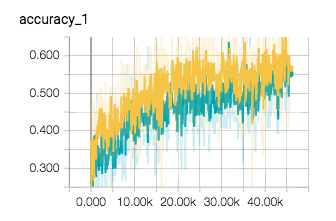
\includegraphics[width=\linewidth]{accuracy.png}
  \caption{Training Accuracy (Yellow: 15words, Green: 300words)}
  \label{fig:accuracy}
\end{figure}

\begin{figure}
  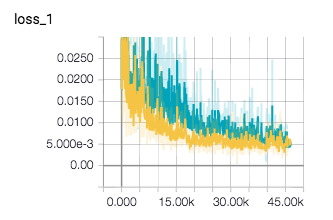
\includegraphics[width=\linewidth]{loss.png}
  \caption{Training Loss (Yellow: 15words, Green: 300words)}
  \label{fig:loss}
\end{figure}

\section{Results}
The model performs well as shown in the table below considering the 
limited amount of training data. The model performs significantly better 
than a representative baseline model that predicts out of 10 classes.

\begin{table}[h]
\begin{center}
\begin{tabular}{|l|rl|}
\hline \bf Model & \bf Accuracy (\%) \\ \hline
Baseline 
(Tf-Idf | 2 class) & 54.5 \\
Tf-Idf (10 Class) & 40.8 \\
Seiamese Network 
(15 words 10 class) & 52.4 \\
Seiamese Network 
(300 words 10 class) & 45.2 \\
\hline
\end{tabular}
\end{center}
\end{table}

We further analyze the classification error rate as the difference between
the expected similarity decile bin and the predicted similarity decile bin.
For example, a pair of songs with 0.83 similarity will have the class as 8.
If the predicted similarity is 0.67 then the prediction will have the class 
6 and the error in prediction is $8-6=2$. Since the similarity  measure is
continuous $\in [0,1]$ we can do the above calculation to see how off the 
similarity predictions were.
\begin{figure}
  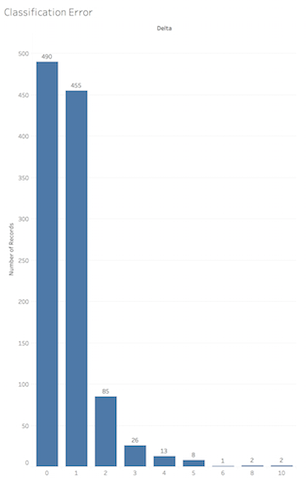
\includegraphics[width=\linewidth]{error.png}
  \caption{Similarity Prediction Error}
  \label{fig:error}
\end{figure}
As can be seen in the figure above the model does a admirable job in 
determining similarity of songs. Almost 50 percent error fall in off
by 1 category which could be easily rectified by training with additional
data resulting in an overall accuracy of \textbf{87.2\%}.

We now divert our attention to a new dataset comprising of 2015 Billboard
Top 100 songs. We pass this data through the model to get the song's
matrix representations. Following this we run principle component analysis
(PCA) on the representations to generate the following graph.
\begin{figure}
  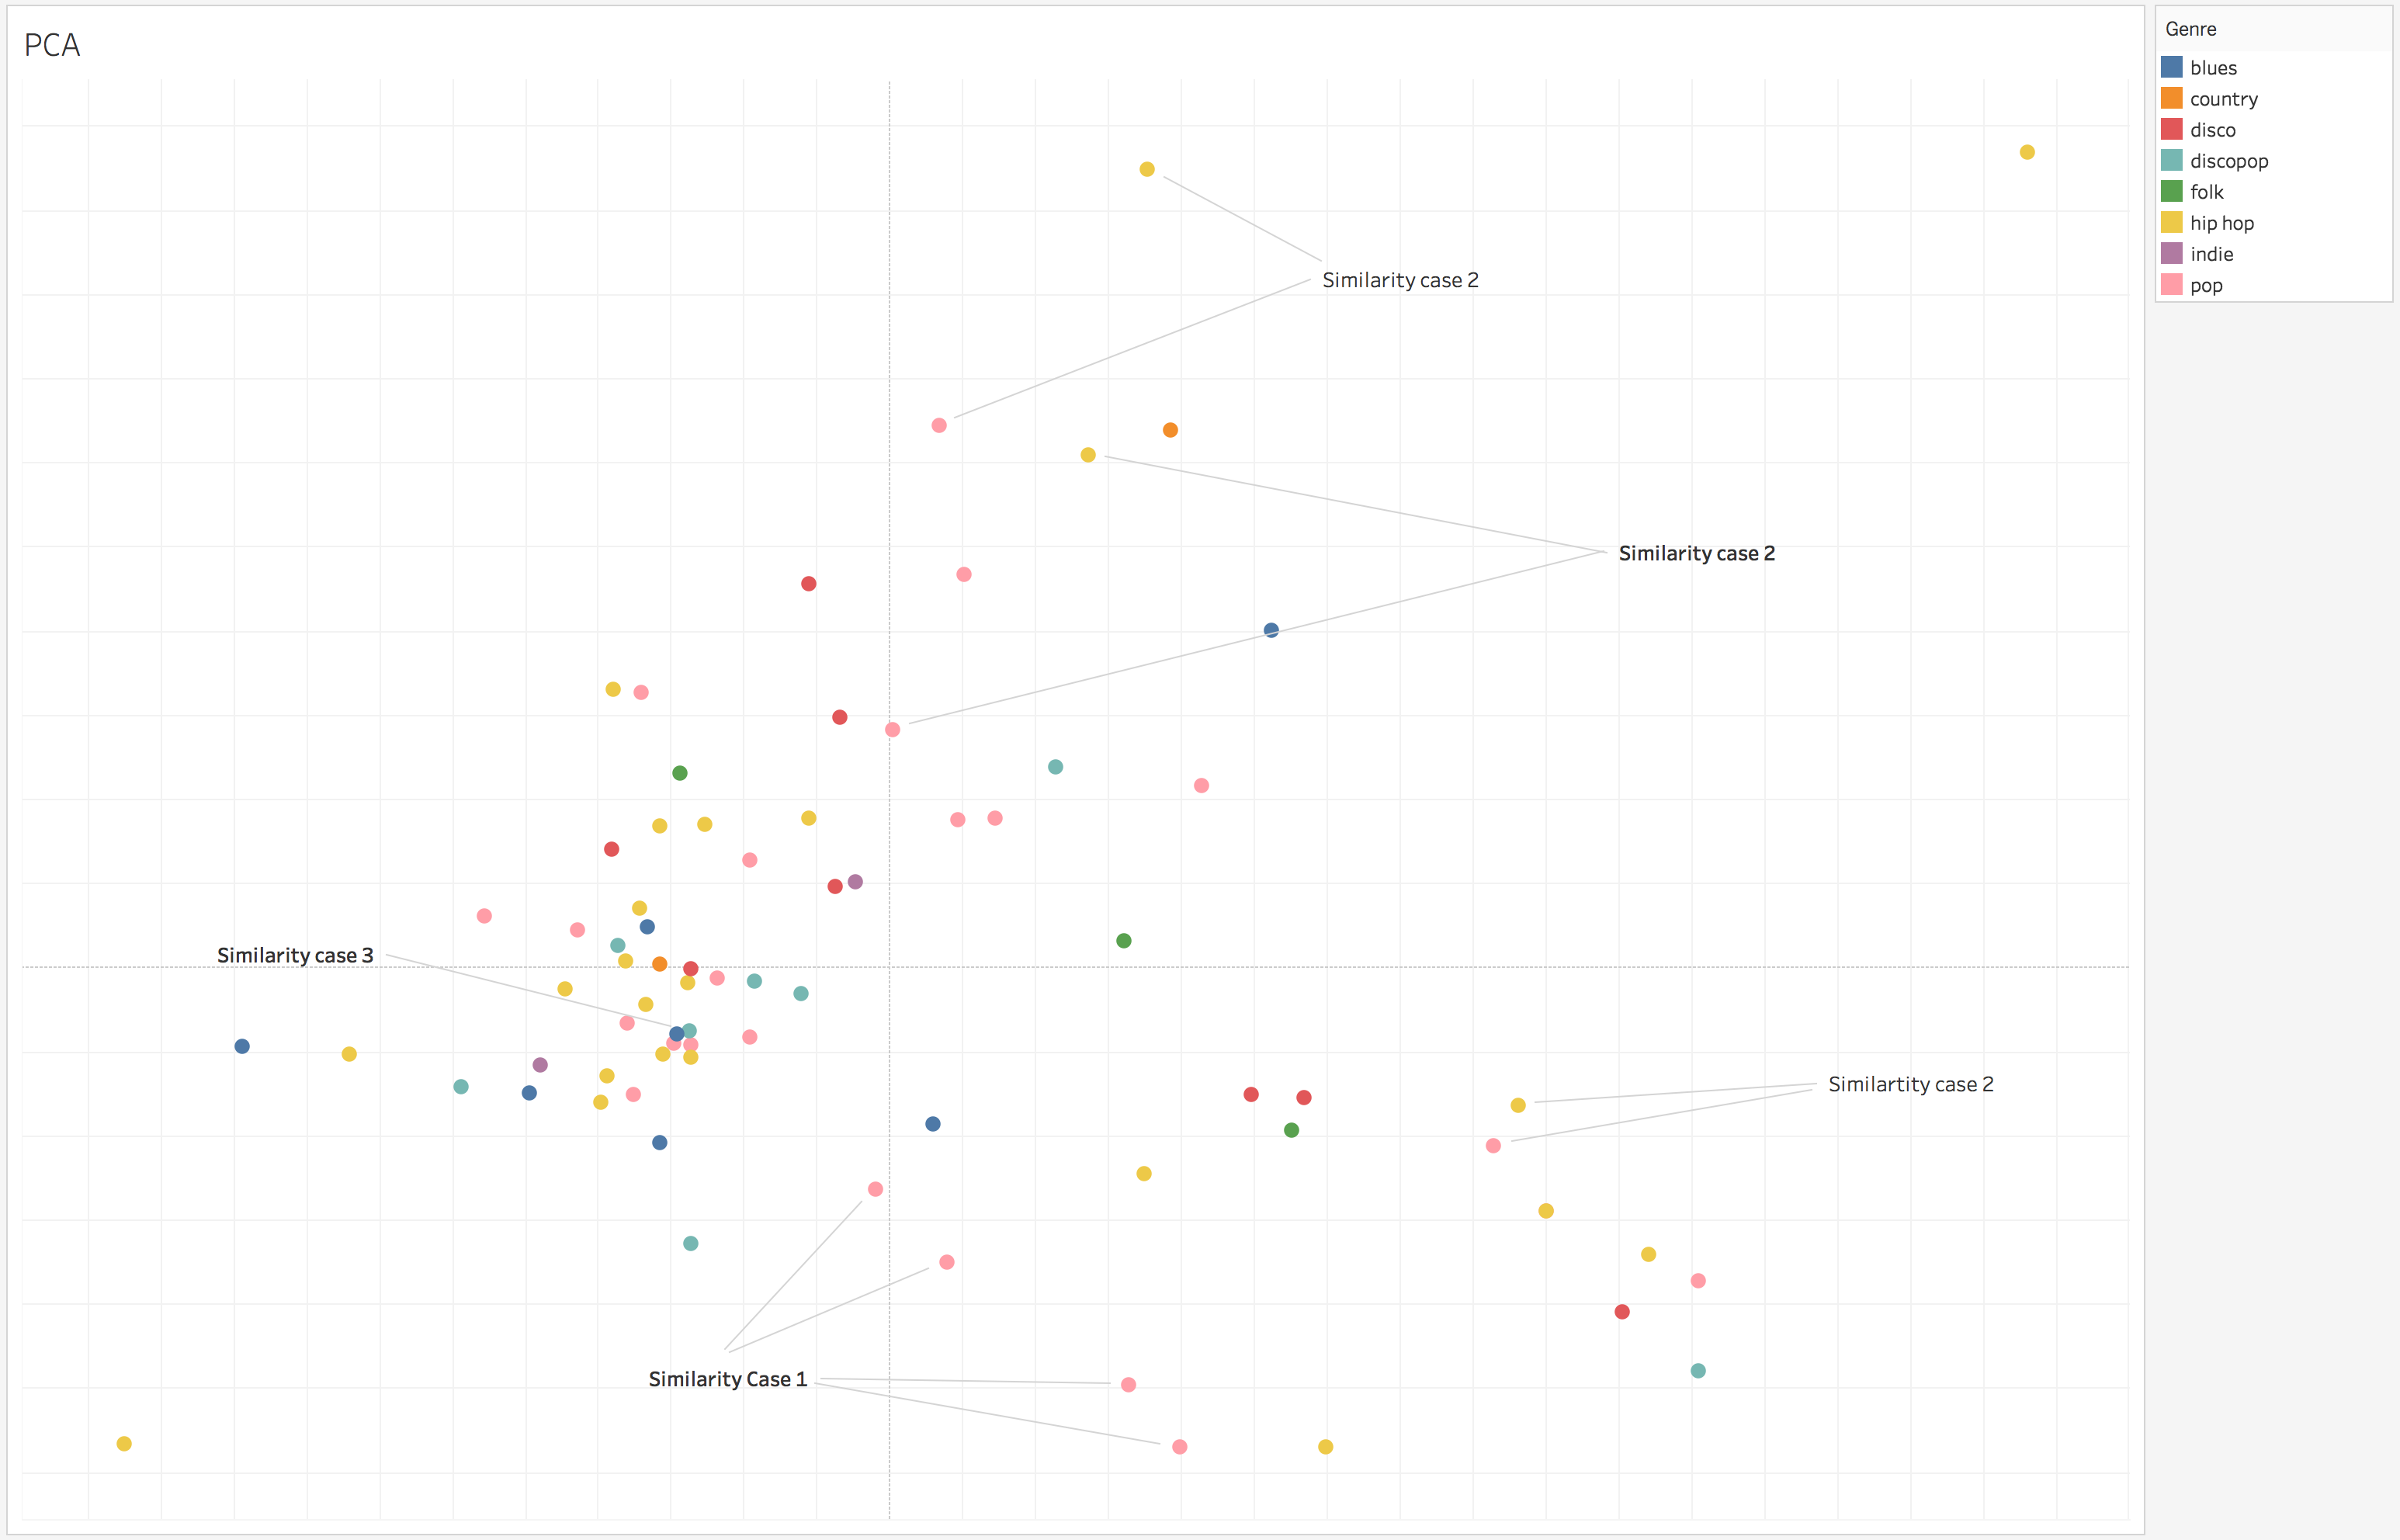
\includegraphics[width=\linewidth]{pca.png}
  \caption{2015 Billboard Top 100 Songs}
  \label{fig:pca}
\end{figure}
From the above graph we can discern that the model can learn semantic
understanding of songs within the same genre (similarity case 1) and 
across genre (similarity case 2 for pop \& hip hop). Further the model is 
able to cluster similar songs across multiple genre (4 in similarity case 3)
which can be very useful in recommendations and in finding formulaic songs.

\section{Conclusion}
The Siamese Recurrent Neural Network based model for analyzing lyrical
similarities shows a 45.2\% validation accuracy. With a larger dataset,
the model can easily reach 87.2\% validation accuracy.

The model performs significantly better than TF-IDF based baseline model
and is also able to learn semantic relationships in songs.

Future work with larger datasets and datasets comprising of other 
languages could result in finding similarities in songs across the globe. 




% include your own bib file like this:
%\bibliographystyle{acl}
%\bibliography{acl2015}
\begin{thebibliography}{}

\bibitem[\protect\citename{Mueller, J., and Thyagarajan, A.}2016]{Mueller:16}
Mueller, Jonas, and Aditya Thyagarajan.
\newblock 2016.
\newblock {\em Siamese Recurrent Architectures for Learning Sentence Similarity}.
\newblock AAAI (pp. 2786-2792)

\bibitem[\protect\citename{Mikolov \bgroup et al.\egroup }2013]{Mikolov:13}
Mikolov, T., Sutskever, I., Chen, K., Corrado, G. S., \& Dean, J.
\newblock 2013.
\newblock Distributed representations of words and phrases and their compositionality.
\newblock {\em Advances in neural information processing systems },
  (pp. 3111-3119).

\bibitem[\protect\citename{Fell, M., and Sporleder, C.}2014]{Fell:14}
Fell, Michael, and Caroline Sporleder.
\newblock 2014.
\newblock {\em Lyrics-based Analysis and Classification of Music}.

\bibitem[\protect\citename{Balakrishnan, A., and Dixit, K}2016]{Balakrishnan:16}
Balakrishnan, Anusha, and Kalpit Dixit.
\newblock 2016.
\newblock {\em DeepPlaylist: Using Recurrent Neural Networks to Predict Song Similarity.}.

\bibitem[\protect\citename{Hochreiter, S., and Schmidhuber, J.}1997]{Hochreiter:97}
Hochreiter, Sepp, and Jürgen Schmidhuber.
\newblock 1997.
\newblock {\em Long short-term memory}.
\newblock Neural computation.

\end{thebibliography}

\end{document}
